\chapter{aCoral结构}

\section{aCoral系统结构}
aCoral由内核(kernel)和外围模块(Peripheral)两大部分组成。
其中内核又包含中断管理系统、内存管理系统、线程管理系统和线程交互系统;
外围模块包括驱动管理、图形用户界面(GUI)、文件系统和网络模块(Net)。
如图2-1所示。

\begin{figure}[htb]
	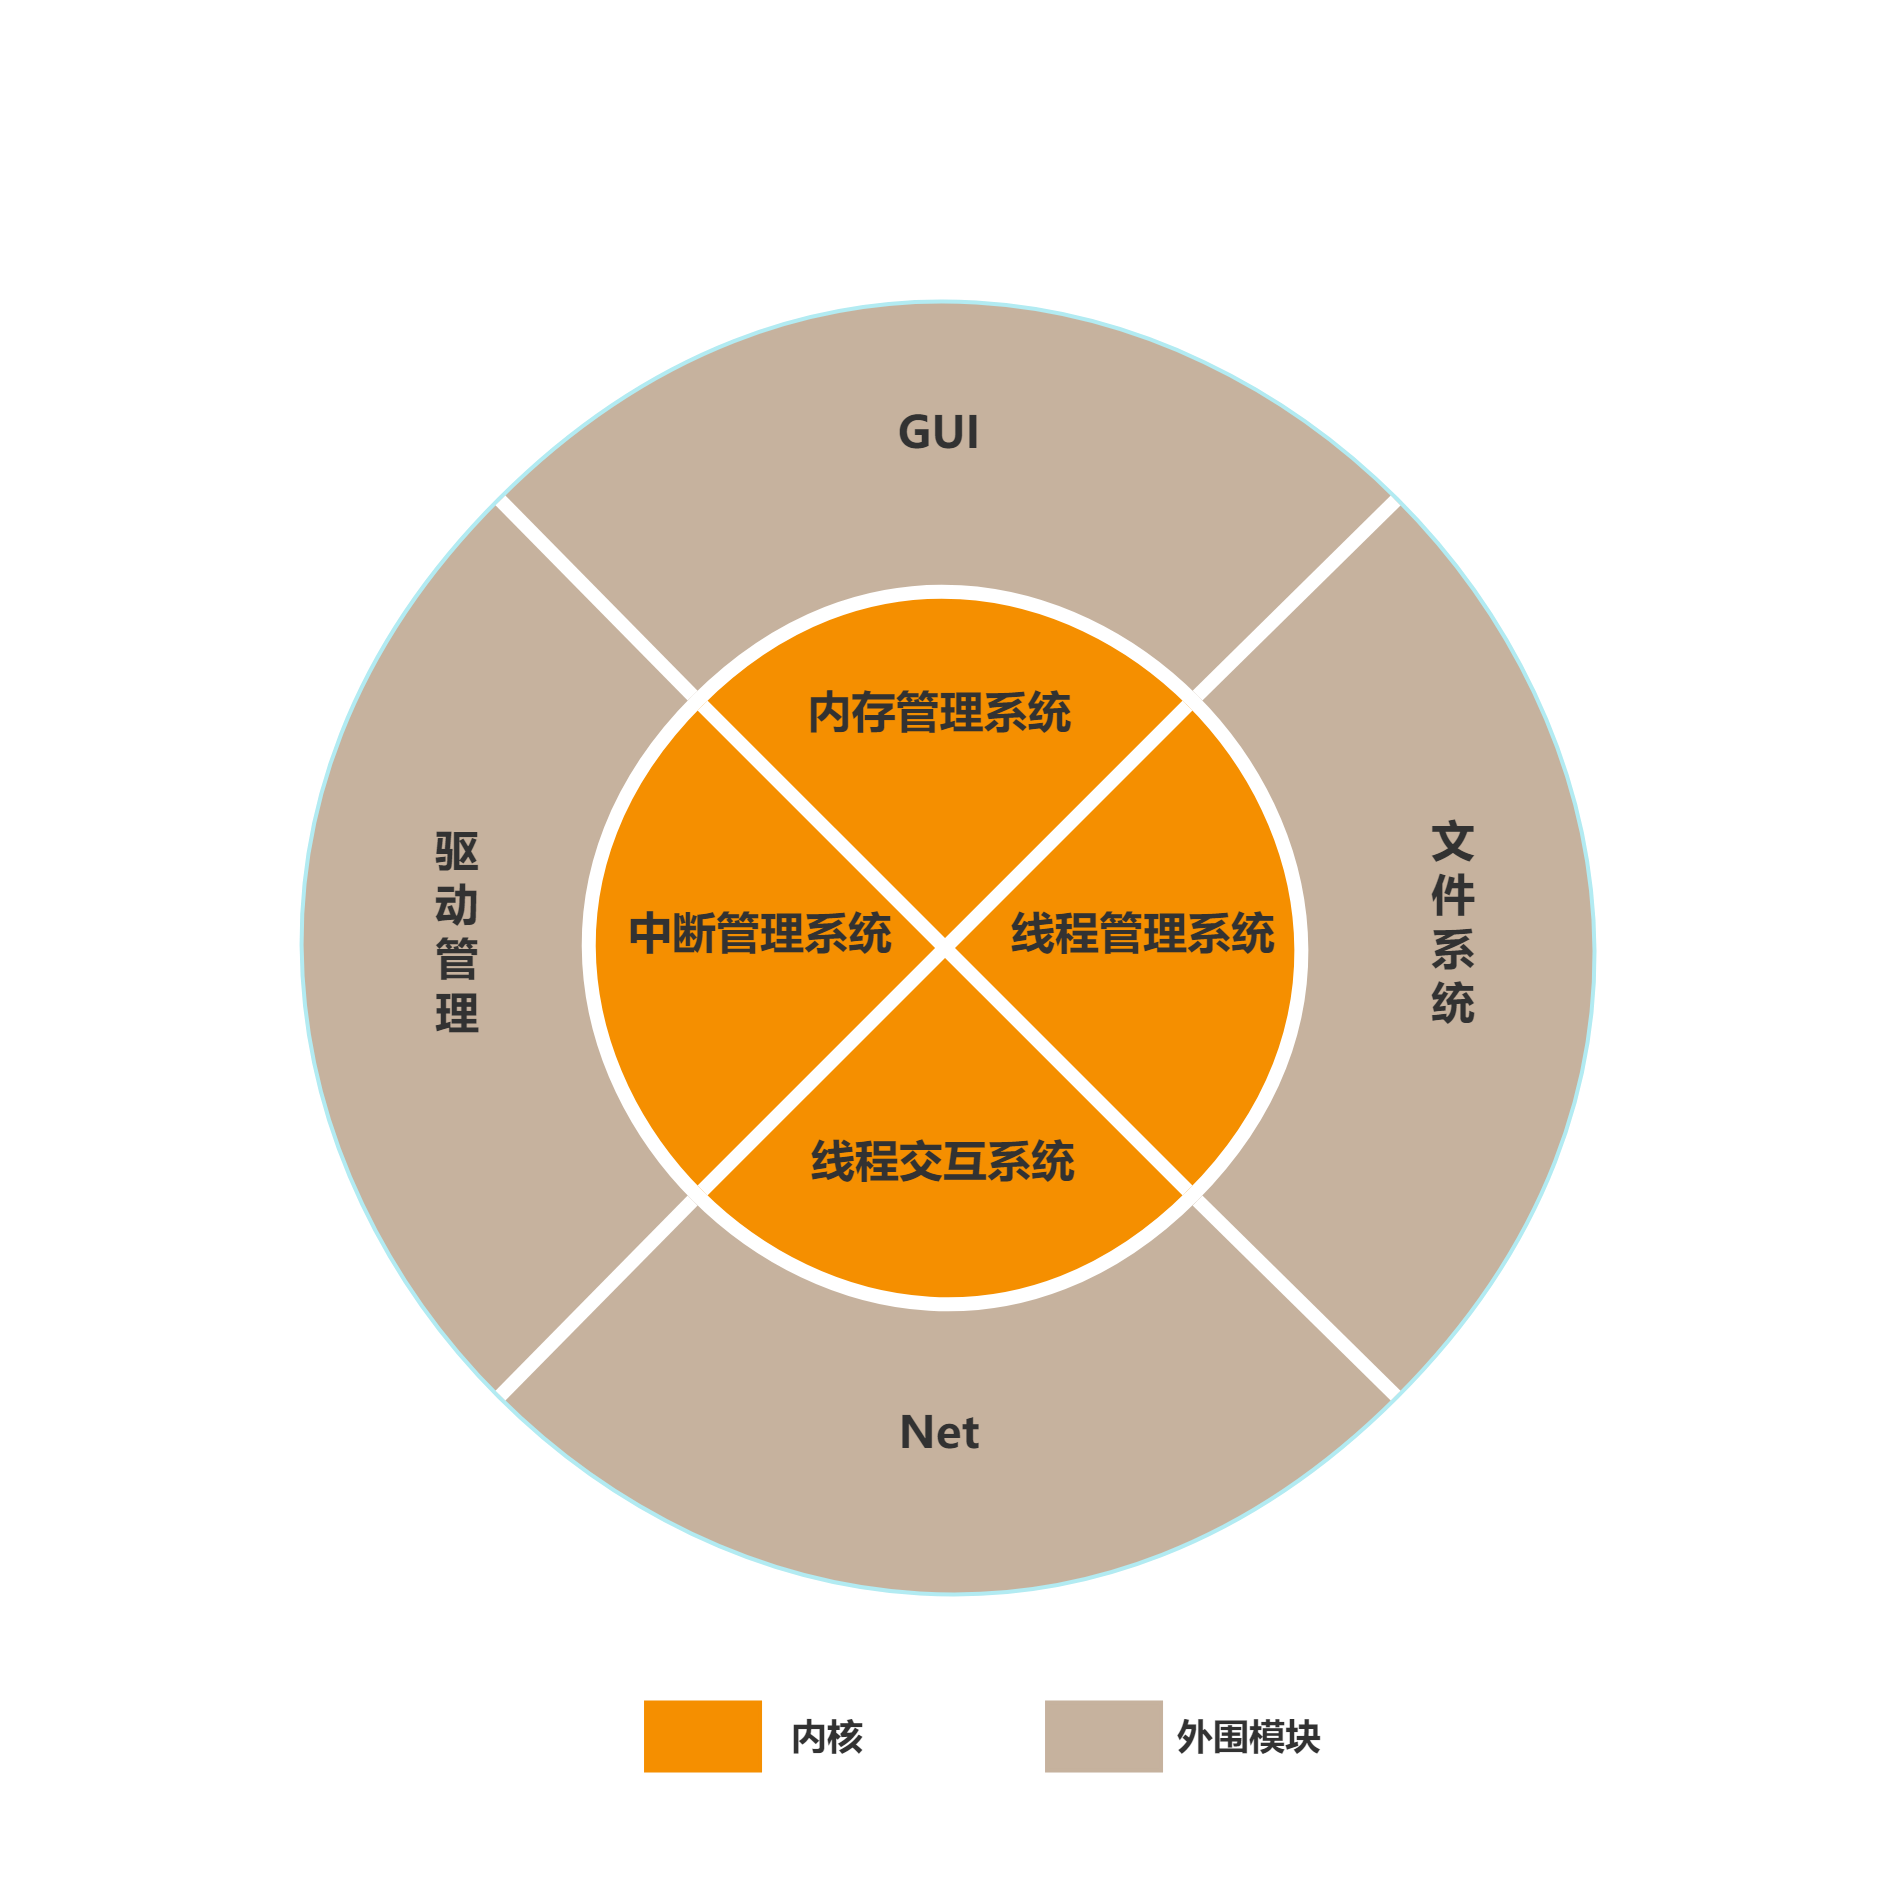
\includegraphics[width=400pt]{aCoral系统结构.png}
	\caption{aCoral系统结构}
	\label{pica}
\end{figure}

内核当中,中断管理系统负责响应并处理处理来自外部和内部的所有中断(异常),例如时钟中断、按键中断等;
内存管理系统负责对mini2440上的SDRAM内存进行管理,包括内存的分配、回收算法的实现;
线程管理系统包括线程调度机制和线程调度策略两个部分,负责创建、挂起、杀死线程等操作以及按照何种策略来调度线程;
线程交互系统包括互斥量、信号量、邮箱、消息队列等线程间交互机制。

\section{aCoral文件结构}
